% !TEX encoding = UTF-8 Unicode

\documentclass{article}

\usepackage{a4wide}
\usepackage[utf8]{inputenc}
\usepackage[T1]{fontenc}
\usepackage[french]{babel}
\usepackage[babel=true]{csquotes} % guillemets français
\usepackage{graphicx}
\graphicspath{{Images/}}
\usepackage{color}
\usepackage{hyperref}
\hypersetup{colorlinks,linkcolor=,urlcolor=blue}

\usepackage{amsmath}
\usepackage{amssymb}


\title{Création de Threads et Interface Graphique}
\author{\'Joan RAVALOMANDA, L3 informatique}
\date{\today}

\begin{document}

\maketitle % pour érire le titre


%% Le résumé:
\begin{abstract}
  Dans ce rapport , je vais vous montrer comment créer un thread , son fonctionnement , la création d'une interface graphique (tKinter ou Swing), et les problèmes rencontrés lors de la réalisation des exercices en python et Java .
\end{abstract}

\section{Introduction}
\label{section:hello} % pour faire référence à  la section ailleurs (\ref{...} voir plus bas)

Un processus est un programme ( fichier exécutable ) en cours d'exécution sur un processeur.
Il est caractérisé par : son code , son espace d'adressage , son ID, sa priorité.
Il est crée lorsqu'un autre processus lance son exécution. 
Les états successifs d'un processus sont généralement représentées par un diagramme d'état.
Tout processus dispose d’un thread principal depuis lequel d’autres threads peuvent être lancés.


Un thread est donc une portion de code capable de s'exécuter en parallèle à d'autres traitements. Ils sont utiles dans bien des cas et parfois même nécessaires comme nous le verrons plus loin dans la section à propos de Swing (Interface Graphique)


Dans un premier temps, nous allons voir la notion de Thread. Ensuite , nous parlerons d'interface graphique et puis nous finirons par voir ces notions dans 2 exercices en Java et en Python.

\section{Thread}
\subsection{Qu'est-ce que c'est ?}
Un Thread est un fil d'exécution de code à l'intérieur d'un processus et qui a la possibilité d'être ordonnancé (sous-processus). Le principal avantage des threads est de pouvoir répartir différents traitements d'un même programme en plusieurs unités distinctes pour permettre leurs exécutions "simultanées".

\subsection{JAVA}
Un thread en Java est un objet, qui doit étendre la classe Thread. Comme Java ne supporte pas l'heritage multiple, il n'est pas toujours possible d'étendre cette classe.
Tout programme Java comporte au moins un thread principal correspondant a la methode main. 
Ci dessous ,on a le code courant du thread de la classe Main.

\begin{verbatim}
public class Main {
   public static void main(String[] args) {
      System.out.println("Hello World!");
   }
}
\end{verbatim}
Ce code affiche tout simplement un message : Hello World!

\subsection{Python}
Pareil en Python, il comporte au moins un thread principal correspondant au thread de contrôle initial du programme. 

Le module threading fournit la classe Thread pour creer et gerer des threads.

Pour créer un thread, il suffit de surcharger la méthode run de la classe Thread. Si le thread a besoin de données lors de son exécution, il faut surcharger son constructeur sans oublier d’appeler le constructeur de la classe mère. L’exécution de thread commence par la création d’une instance et l’appel à la méthode start. En résumé, il faut :

\begin{itemize}
\item surcharger la classe \verb|threading.Thread|,
\item surcharger le constructeur sans oublier d’appeler le constructeur \verb|threading.Thread.__init__|
\item surcharger la méthode \verb|run|, c’est le code que devra exécuter le thread,
\item créer une instance de la nouvelle classe et appeler la méthode \verb|start| pour lancer le thread secondaire qui formera le second fil d’exécution.
\end{itemize}
\begin{center}
  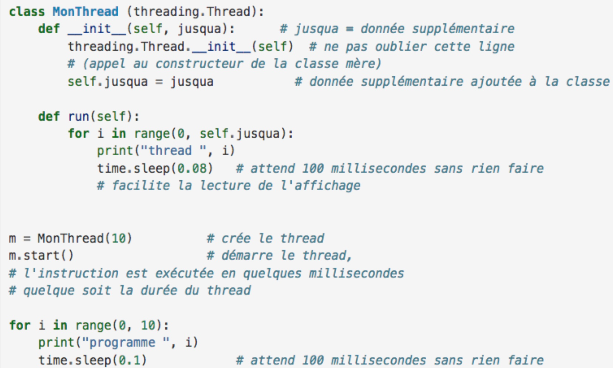
\includegraphics[scale=0.5]{thread.png}
\end{center}

Le programme affiche des lignes qui proviennent du thread principal et du thread secondaire dont les affichages diffèrent, ce qui donne :

\begin{center}
  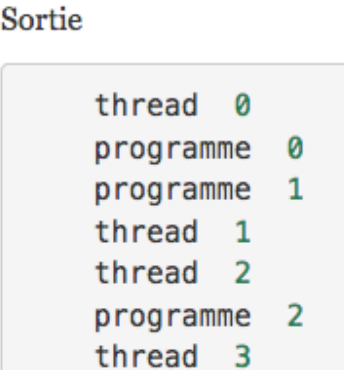
\includegraphics[scale=0.5]{threadS.png}
\end{center}

\section{Interface Graphique}
Une interface graphique (GUI: Graphical User Interface) ou un environnement graphique est un dispositif de dialogue homme-machine, dans lequel les objets à manipuler sont dessinés sous forme de pictogrammes à l'écran, de sorte que l'usager peut utiliser en imitant la manipulation physique de ces objets avec un dispositif de pointage, le plus souvent une souris.

\subsection{Java}
Swing fait partie de la bibliothèque Java Foundation Classes (JFC). C'est une API dont le but est similaire à celui de l'API AWT mais dont les modes de fonctionnement et d'utilisation sont complètement différents. Swing a été intégré au JDK. 

La bibliothèque JFC contient : 

\begin{itemize}
\item L'API Swing : de nouvelles classes et interfaces pour construire des interfaces graphiques
\item Accessibility API
\item 2D API: support du graphisme en 2D
\item API pour l'impression et le cliquer/glisser
\end{itemize}

Les composants Swing forment un nouvelle hiérarchie parallèle à celle de l'AWT. L'ancêtre de cette hiérarchie est le composant JComponent.
La procédure à suivre pour utiliser un composant Swing est identique à celle des composants de la bibliothèque AWT : créer le composant en appelant son constructeur, appeler les méthodes du composant si nécessaire pour le personnaliser et l'ajouter dans un conteneur.

Swing utilise la même infrastructure de classes qu'AWT, ce qui permet de mélanger des composants Swing et AWT dans la même interface.

La classe de base d'une application est la classe JFrame. Son rôle est équivalent à la classe Frame de l'AWT et elle s'utilise de la même façon. 

Code d'une simple fenêtre en Java:
\begin{verbatim}
import javax.swing.*;
import java.awt.event.*;

public class Swing1 extends JFrame {

   public Swing1() {
      super("SESAME OUVRE-TOI");

      WindowListener l = new WindowAdapter() {
         public void windowClosing(WindowEvent e){
            System.exit(0);
         }
      };

      addWindowListener(l);
      setSize(200,100);
      setVisible(true);
   }

   public static void main(String [] args){
      JFrame frame = new Swing1();
   }
}
\end{verbatim}

Résultat: Une fenêtre s'ouvre...
\begin{center}
  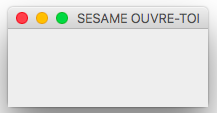
\includegraphics[scale=0.5]{fenetreJ.png}
\end{center}

\subsection{Python}

Comment créer des interfaces graphiques à l'aide d'un module présent par défaut dans Python : Tkinter ?

Tkinter (Tk interface) est un module intégré à la bibliothèque standard de Python, bien qu'il ne soit pas maintenu directement par les développeurs de Python. Il permet de créer des interfaces graphiques.


De nombreux composants graphiques (ou widgets) sont disponibles : 
\begin{itemize}
\item fenêtre (classe Tk), \item bouton (classe Button), \item case à cocher (classe Checkbutton), \item étiquette (classe Label), \item zone de texte simple (classe Entry), \item menu (classe Menu), \item zone graphique (classe Canvas), \item cadre (classe Frame)...
\end{itemize}

Code d'une simple fenêtre en Python :
\begin{verbatim}
from tkinter import *

Fenetre = Tk()

bouton=Button(Fenetre, text="quitter", command=Fenetre.destroy)

bouton.pack()

Fenetre.mainloop()
\end{verbatim}

\begin{center}
  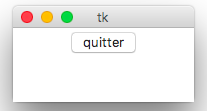
\includegraphics[scale=0.5]{fenetreP.png}
\end{center}


Particularité de cette fenêtre: Ce code crée une fenêtre contenant un bouton "Quitter". Lorsqu'on va cliquer dessus, la fenêtre va se fermer.

\section{File entiers }

Ce qui nous ai demandé dans cet exercice est de crée une file d'entiers , un thread producteur et un thread consommateur se partageant cette file et répétant indéfinement les actions :
\begin{itemize}
\item Producteur : Ajout d’un entier choisi aleatoirement entre 1 et 100 puis repos. Si la file est pleine, ce thread est mis en attente jusqu’a ce qu’une place soit disponible.
\item Consommateur : Retrait d’un entier, affichage de cet entier puis repos. Si la file est vide, le thread est mis en attente jusqu’a ce qu’un entier soit disponible.
\end{itemize}

Résultat obtenu : 
\begin{center}
  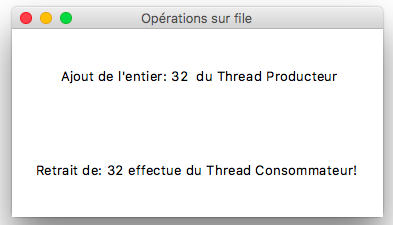
\includegraphics[scale=0.5]{2_3.png}
\end{center}

Il était demandé aussi que les threads soient interrompus lorsqu'on appuie sur la touche return.
J'ai eu du mal à le faire. Généralement, sauf erreur de ma part, on utilise input("") pour python3, dans le main, pour qu'on stoppe les threads en cliquer sur la touche entrée mais ca ne fonctionner pas pour moi.

Du coup, il fallait que je crée une fonction Clavier en passant par un évènement 

Résultat obtenu : 
\begin{center}
  \includegraphics[scale=0.5]{Clavier.png}
\end{center}

 
\section{Balle En Mouvement }

Ici, il était demandé d'afficher des balles en mouvements dans une fenêtre avec plusieurs caractéristiques en plus (start, stop, ajout de balle, suppression de balles, collision des balles, affichage du score, d'une horloge). J'ai pas pu finir cet exercice. Voila ce que j'ai pu réalisé :

\begin{center}
  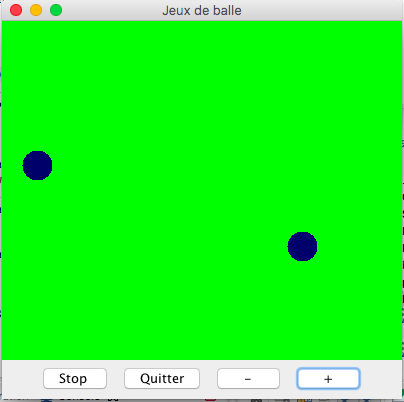
\includegraphics[scale=0.5]{balle.png}
\end{center}


Il me manque les collision, l'horloge et le score.




\begin{thebibliography}{9}
\bibitem{wiki}
         Wikipedia : \url {https://fr.wikipedia.org/wiki/Interface_graphique}
 \bibitem{eve}       
         Notion d'évènement : \url {http://tkinter.fdex.eu/doc/event.html}
\bibitem{opcl}
	Thread, Fenetre, GUI : \url{http://openclassrooms.com/}
\end{thebibliography}

	
	

\end{document}
